\documentclass[11pt]{article}

% If you're new to LaTeX, here's some short tutorials:
% https://www.overleaf.com/learn/latex/Learn_LaTeX_in_30_minutes
% https://en.wikibooks.org/wiki/LaTeX/Basics

% Formatting
\usepackage[utf8]{inputenc}
\usepackage[margin=1in]{geometry}
\usepackage[titletoc,title]{appendix}
\usepackage{indentfirst}
% Math
% https://www.overleaf.com/learn/latex/Mathematical_expressions
% https://en.wikibooks.org/wiki/LaTeX/Mathematics
\usepackage{amsmath,amsfonts,amssymb,mathtools}
\usepackage{tikz}
\usetikzlibrary{calc}

\usepackage{csquotes}
\usepackage{tabularx}

% Images
% https://www.overleaf.com/learn/latex/Inserting_Images
% https://en.wikibooks.org/wiki/LaTeX/Floats,_Figures_and_Captions
\usepackage{graphicx,float}

% Tables
% https://www.overleaf.com/learn/latex/Tables
% https://en.wikibooks.org/wiki/LaTeX/Tables

% Algorithms
% https://www.overleaf.com/learn/latex/algorithms
% https://en.wikibooks.org/wiki/LaTeX/Algorithms
\usepackage[ruled,vlined]{algorithm2e}
\usepackage{algorithmic}

\usepackage{setspace}
\doublespacing

\usepackage{pdfpages}

\interfootnotelinepenalty=10000

% References
% https://www.overleaf.com/learn/latex/Bibliography_management_in_LaTeX
% https://en.wikibooks.org/wiki/LaTeX/Bibliography_Management
\usepackage[notes,backend=biber]{biblatex-chicago}
\addbibresource{bibliography.bib}

% Title content
\title{\vspace{-3cm}FBI: Mastermind Project Report}
\author{Chen Stanilovsky, Rinchen Lama, Michelle Lucero\\Artificial Intelligence, CUNY Hunter College}
\date{May 10, 2021}

\begin{document}
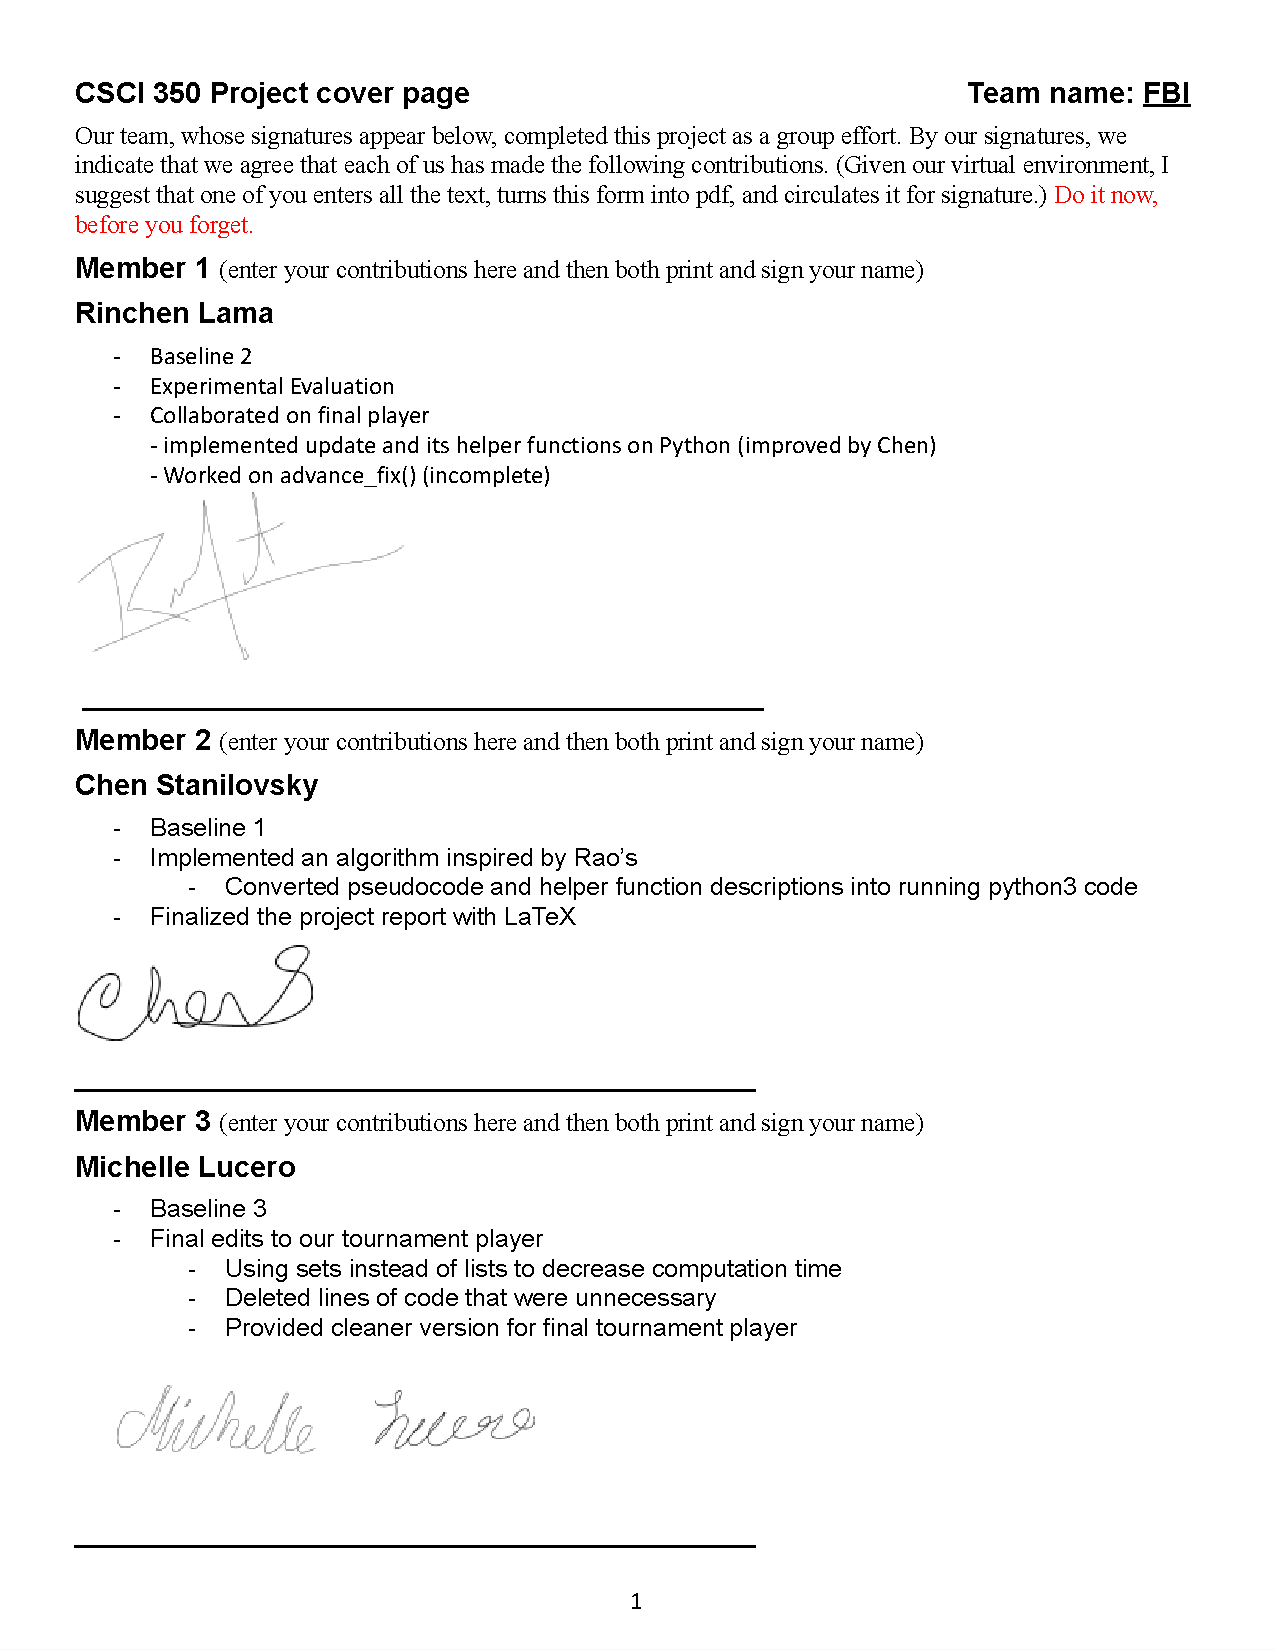
\includepdf[pages=-]{cover_letter}
\maketitle
    \section{Intro}
    
    Mastermind is a game that involves two players: a code maker and a code breaker. Usually the game consists of code pegs of six different colors and four key holes that consist of any combination of those six code pegs. The code maker is in charge filling the four keyholes with any combination of the available six color pegs. The code breaker has a limited amount of guesses they can make. After each guess, the code maker must reply with the number of bull and cows the code breaker’s guess contained. The number of bulls signifies the number of correct colors in the correct position. The number of cows signifies the number of correct colors in the wrong position. The secret code made by the code maker has to be guessed correctly by the code breaker in the given amount of tries.
    
    For this project, we were tasked with creating an algorithm that is capable of breaking the code in any size game given a hundred guesses and 5 seconds to get it right.
    
    \section{Background Reading}

    Due to the fact that this game was new to all the team members, we had to read the rules and give ourselves some time to formulate various strategies. We found an online website that both described the game and had a good description of the rules \autocite{rules}. In this online version of the game, the only option was to play with 6 pegs and 8 colors. Unlike the tournament, this version only allowed 10 guesses and the colors were non repeating. 
    
    Naively enough, our initial strategy as a group was to try sets of completely different colors in the initial guess and then slowly infer from the response. We were quick to assume that the game would be best played by an agent that would perform some sort of local search. However, as we discussed strategies further, we realized that local search would not be efficient. Upon reviewing T. Mahadeva Rao's algorithm\autocite{rao}, we realized that infer from responses is indeed useful and can allow us to improve our guesses.

    We used the algorithm to complete a few games on the website and quickly realized that Rao's algorithm was a good place to start. The algorithm works by maintaining lists of colors deemed to be part of the answer along with their possible positions. We recreated the behavior of the algorithm many times on the website\autocite{webgames} which allowed our team to grow an understanding of how the algorithm behaves in various situations.

    One thing we noted was that as the number of pegs and colors increases, the more computationally expensive it becomes to break the code. Given 100 guesses and up to 26 possible colors ('A'-'Z'), Rao’s algorithm would consistently find the solution as long as the board size was less than 74. This stems from the time complexity of this algorithm: O(T) = m+n, where m is the board size and n is the number of colors. With this in mind, we decided to make use of a knowledge base, consisting of inferences, so our algorithm could gain knowledge from the code maker’s response. We used Rao’s algorithm as the basis of our algorithm, however we made certain changes to improve its runtime, which will be discussed later in this paper. As a result, we were able to design a general player that can guess codes efficiently independent of which secret-code selection algorithm (SCSA) was used.

    Due to the linear nature of Rao's Algorithm's time complexity, it is a scalable option for us.

    \section{Our Implementation}

    Our team didn’t focus on constructing guesses for any particular SCSAs. This is because we wanted an algorithm which was efficient and a complete, given enough guesses. While we could possibly prepare an agent that would strategize differently for each SCSA, we realized that it would mean looking at the mystery codes for hours on end. On the other hand, a well built general purpose player would let us focus more on finding the solution efficiently instead of worrying about each possible SCSA we could encounter. Further, since some SCSAs were completely unobservable, we would need to prepare a general strategy to tackle them anyway.

    Our algorithm was heavily influenced by Rao’s algorithm, which has the primary functions of updating a list of inferences (based on responses) and generating new guesses. However, the article describing the algorithm did not provide any pseudo-code for sub-routines involved in its primary functions. Due to this, we had to be clever about how we went about implementing the algorithm if we wanted to keep the efficient time complexity. 
    
    One enhancement to the original pseudo-code we made was introducing a new data structure into our implementation. Rao's algorithm \enquote{uses a simple list data structure to represent the knowledge gained}\autocite{rao}. Our algorithm also makes use of a simple list, but we combine it with a set data structure to track the positions which have been fixed to a color. A set works because two different positions cannot be the same position, therefore we do not lose information using a set. This improvement allows for us to determine how many and which positions are fixed in constant time. Without the set, these operations take linear time as we would only have access to an array without knowing which colors have been fixed. 
    
    One change which our team hoped to make but could not implement in time, was a method called \enquote{Advance Fix}. During our guesses, we maintain an array of inferences, which in each row contains a color and list of possible positions for that color. An insight that we had was that if multiple rows in inferences share the same letter, we can shrink down the number of positions of subsequent rows. Let's say we have two rows with the color 'A'. If the both A's have 0 as their first possible position, the second A will never be placed in position 0. If the first A belong in position 0 then the second A cannot. If the first A doesn't belong in position 0, then neither will the second A. This improvement would take place in the clean up function and would have to run multiple times. By running it multiple times, we can extend this shrinkage to 3+ rows of the same color.

    \section{Constructing Guesses}
    Due to the fact that our algorithm was based on Rao's algorithm, the process of constructing guesses will be similar to the ones described in the article\autocite{rao}. We will now go through an example to show how our algorithm constructs its guesses.

    Let's assume are playing a 5 peg-7 color game where the secret code is \enquote{GCEED}. Let R be the response from the code maker, BF be the index in the inferences which is being fixed, BC be the color being considered, I be the inferences list, F be the fixed positions set, and G be the the guess of the codebreaker. The response contains three numbers in the following order, the number of bulls, the number of cows, and the number of guesses made so far.\\

    \noindent R: (0, 0, 0), BF = -1, BC = 'A', F: $\emptyset$

    \noindent I: $\emptyset$

    The algorithm starts off by guessing the color ‘A’ which is being considered. Since it is the first guess and doesn’t contain any inferences, the guess is naive and consists of the color being considered multiplied by the board length. Since the color 'A' is not part of the code, our response indicates no cows or bulls.

    \noindent G: \enquote{AAAAA}

    \noindent R: (0, 0, 1), BF = -1, BC = 'B', F: $\emptyset$

    \noindent I: $\emptyset$

    Each time a guess is made, we increase the value of the character which is being considered. Using ASCII math, we add 1 to the character 'A' and being considered becomes 'B'. Since we did not gain any inferences from the first guess, we will make another naive guess of all B's.

    \noindent G: \enquote{BBBBB}

    \noindent R: (0, 0, 2), BF = -1, BC = 'C', F: $\emptyset$

    \noindent I: $\emptyset$

    Since 'B' is not part of the answer, we repeat the same process: increase being considered to 'C' and try the naive guess again.\\

    \noindent G: \enquote{CCCCC}

    \noindent R: (1, 0, 3), BF = 0, BC = 'D', F: $\emptyset$

    \noindent I: \begin{tabularx}{.25\textwidth}{|X|}
        \hline
        Color, [Positions]\\\hline 
        'C', [0, 1, 2, 3, 4]\\\hline
    \end{tabularx}\\
    
    The response now indicates a single bull, which indicates to us that a single C belongs somewhere in the code. However, we cannot immediately deduce its positions since it could be any of the positions tried. 
    When our algorithm discovers a color that belongs in the answer, it adds the corresponding amount of rows to the inferences. The number of rows to add is calculated in two different ways. If inferences is empty, bulls + cows, otherwise, (bulls + cows) - \# of positions fixed to a color - 1.

    From this point on our guesses will consist of 3 things: fixed positions will always be filled in with the color they are fixed to, the color being fixed will be placed in its next possible position, all other positions will be filled with the color being considered. The color being fixed is indicated by an index into the inferences. When we first add a color to inferences, we set being fixed to 0. After that, each time we fix the color that is being fixed, we update being fixed to be the index of the next color to be fixed from inferences (in order).

    Therefore, our next guess will have C in position 0 and the rest will be D's.\\

    \noindent G: \enquote{CDDDD}

    \noindent R: (1, 1, 4), BF = 0, BC = 'E', F: $\emptyset$

    \noindent I: \begin{tabularx}{.4\textwidth}{|X|X|}
        \hline
        Color, [Positions]&\\\hline 
        'C', [1, 2, 3, 4] &'D'  [0, 1, 2, 3, 4]\\\hline
    \end{tabularx}\\
    
    The response was 1 bull and 1 cow which causes us to add a single list for D due to the formula, (bulls + cows) - \# fixed - 1 = (1 + 1) - 0 - 1 = 1. Now we need to determine if the bull was for the C or D. If C is a bull, that means that one of the D's was a cow so it needs to be placed in some position that wasn't tried. However, the only position that wasn't tried was where C was. Since we assumed C is a bull, D cannot belong there and we get a contradiction. So it can only be the case that C is a cow. For this reason, we remove position 0 from the row for C.

    Our guess will have C in its next position, 1, and the rest will be E's.\\

    \noindent G: \enquote{ECEEE}

    \noindent R: (3, 0, 5), BF = 1, BC = 'F', F: \{1\}

    \noindent I: \begin{tabularx}{.85\textwidth}{|X|X|X|X|}
        \hline
        Color, [Positions]&&&\\\hline 
        'C', [1]&'D', [0, 2, 3, 4]&'E', [0, 2, 3, 4]&'E', [0, 2, 3, 4]\\\hline
    \end{tabularx}\\
    
    This response only included bulls, therefore the color that is being fixed belongs in the position that was tried, which was 1. We fix it in that position and add the position to the fixed set. Since we just fixed the color that was being fixed, we must change the index of being fixed to 1. Also, since 1 bull represents the 'C', the other two indicate to us that two E's belong in the answer so we add those rows. Once we have added all rows and fixed our color, we can clean up inferences. Cleaning up means removing all instances of a fixed position in rows other than the one with the color it is fixed to. In our case, the C in row index 0 is fixed to 1 so we remove 1 from rows 1-3.

    \noindent G: \enquote{DCFFF}
    
    \noindent R: (1, 1, 6), BF = 1, BC = 'G', F: \{1\}

    \noindent I: \begin{tabularx}{.85\textwidth}{|X|X|X|X|}
        \hline
        Color, [Positions]&&&\\\hline 
        'C', [1]&'D', [2, 3, 4]&'E', [0, 2, 3, 4]&'E', [0, 2, 3, 4]\\\hline
    \end{tabularx}\\

    The 1 bull is due to the fixed C, so we can ignore it. The 1 cow is due to the D being in the wrong position. Therefore, F does not belong in the answer and we won't add it to inferences. Since we got a cow for D, it must be in the wrong position so we remove 0 from its positions, update being considered, and make our next guess.

    \noindent G: \enquote{GCDGG}

    \noindent R: (2, 1, 7), BF = 1, BC = 'E', F: \{1\}

    \noindent I: \begin{tabularx}{\textwidth}{|X|X|X|X|X|}
        \hline
        Color, [Positions]&&&&\\\hline 
        'C', [1]&'D', [3, 4]&'E', [0, 2, 3, 4]&'E', [0, 2, 3, 4]&'G', [0, 2, 3, 4]\\\hline
    \end{tabularx}\\

    In this step, we know that one of the bulls is 'C', so D and G are one bull and one cow. Following from the same logic from when we had 1 bull and 1 cow earlier, if D is a bull, then G is a cow which cannot be placed in any new positions. Due to the contradiction, D must be a cow and G is a bull. For these reasons, we add G to inferences and we remove position 2 from D. Now that inferences is the same length as the number of positions, being considered will always be the color of a row in inferences that comes after the color being fixed and isn't already fixed.
    
    \noindent G: \enquote{ECEDE}

    \noindent R: (2, 2, 8), BF = 3, BC = 'G', F: \{1, 3, 4\}

    \noindent I: \begin{tabularx}{\textwidth}{|X|X|X|X|X|}
        \hline
        Color, [Positions]&&&&\\\hline 
        'C', [1]&'D', [4]&'E', [3]&'E', [0, 2]&'G', [0, 2]\\\hline
    \end{tabularx}\\
    
    We have received a response with 2 bulls and 2 cows. Since the inferences list is the same length as the number of position, we no longer add rows. Therefore, we are left to deal with the two cows. When we have two cows, this indicates that the color that is being considered belongs in the position where the color that is being fixed is. So we fix our E at index 2 to position 3. When we end up cleaning up, 3 gets removed from D and it is only left with 4. Due to this, D gets fixed to 4 and all other 4's in positions are removed. When we go to update being fixed and being considered. We find that the next color to fix is the E in position 3, therefore being considered will be G.

    We build our next guess by assigning fixed positions to their colors and putting E in position 0, leaving only position 2 for G.

    \noindent G: \enquote{ECGED}

    \noindent R: (3, 2, 9), F: \{0, 1, 2, 3, 4\}

    \noindent I: \begin{tabularx}{\textwidth}{|X|X|X|X|X|}
        \hline
        Color, [Positions]&&&&\\\hline 
        'C', [1]&'D', [4]&'E', [3]&'E', [2]&'G', [0]\\\hline
    \end{tabularx}\\

    The 3 bulls which we received were thanks to the 3 fixed positions. Therefore the 2 cows refer to E and G which we are still fixing. Using the same idea as last guess, we fix the color being considered in the position of the color being fixed. This fixed G to position 0. Once we clean up, the final E has no choice but to be fixed in position 2.

    Our final guess is created by assigning each position to the color it was fixed to.

    \noindent G: \enquote{GCEED}
    
    \noindent R: (5, 0, 10) Success!\\[2in]

    % References
    \printbibliography

\end{document}%